% =============================================================================
% Pre-defense presentation --- narrative flow
%   task -> reward -> diffusion-diversity idea -> motivational exhaustive
%   -> reward map -> visual confirmation -> REINFORCE -> 8-exp result -> viz
% =============================================================================
\documentclass[10pt,aspectratio=169]{beamer}

\usetheme{default}
\usecolortheme{default}

\usepackage[T1]{fontenc}
\usepackage{lmodern}
\usepackage{microtype}
\usepackage{graphicx}
\usepackage{booktabs}
\usepackage{amsmath,amssymb}
\usepackage{xcolor}
\usepackage{array}

\definecolor{accent}{HTML}{1F4E79}
\definecolor{accent2}{HTML}{A23B3B}
\definecolor{muted}{HTML}{6E7781}

\setbeamercolor{title}{fg=black}
\setbeamercolor{frametitle}{fg=black}
\setbeamercolor{structure}{fg=accent}
\setbeamercolor{normal text}{fg=black}
\setbeamercolor{alerted text}{fg=accent2}

\setbeamerfont{title}{series=\bfseries, size=\LARGE}
\setbeamerfont{subtitle}{series=\mdseries, size=\large}
\setbeamerfont{frametitle}{series=\bfseries, size=\large}

\setbeamertemplate{navigation symbols}{}
\setbeamertemplate{itemize item}{\color{accent}\textbullet}
\setbeamertemplate{itemize subitem}{\color{muted}\textendash}

\setbeamertemplate{footline}{%
  \hspace{0.8em}%
  \raisebox{-0.2em}{
\includegraphics[height=1.4em]{skoltech_logo.png}}%
  \hspace{0.7em}\textcolor{muted}{\tiny Grozny \textendash\ Exploring Diffusion Trajectories}%
  \hfill\textcolor{muted}{\tiny\insertframenumber\,/\,\inserttotalframenumber}%
  \hspace{0.8em}\vspace{0.35em}%
}

\setbeamertemplate{frametitle}{%
  \vspace{0.55cm}%
  \hspace{-0.1em}\insertframetitle\par%
  \vspace{-0.1cm}%
  \hspace{-0.1em}\textcolor{accent}{\rule{0.12\textwidth}{1.3pt}}\par%
  \vspace{0.25cm}%
}

\setbeamertemplate{title page}{%
  \vspace*{0.6cm}
  \begin{flushleft}
    
\includegraphics[height=1.4em]{skoltech_logo.png}\par
    \vspace{0.5cm}
    {\tiny\textcolor{muted}{MSc Data Science \textendash\ Pre-defense}\par}
    \vspace{0.45cm}
    {\usebeamerfont{title}\inserttitle\par}
    \vspace{0.2cm}
    \textcolor{accent}{\rule{0.35\textwidth}{1.4pt}}\par
    \vspace{0.25cm}
    {\usebeamerfont{subtitle}\textcolor{muted}{\insertsubtitle}\par}
    \vspace{0.9cm}
    {\normalsize\textbf{Student:} Sergey Grozny\par}
    \vspace{0.15em}
    {\normalsize\textbf{Advisor:} Aleksandr Katrutsa, PhD\par}
    \vspace{0.15em}
    {\normalsize\textbf{Co-advisor:} Aibek Alanov, PhD\par}
    \vspace{0.6cm}
    {\footnotesize\textcolor{muted}{April 2026}\par}
  \end{flushleft}
}

\graphicspath{
  {../Skoltech_MSc_Thesis_Template_DS/images/}
  {../Skoltech_MSc_Thesis_Template_DS/images/phase1/}
  {../Skoltech_MSc_Thesis_Template_DS/images/phase2/}
  {./figures/}
}

\newcommand{\key}[1]{\textcolor{accent}{\textbf{#1}}}
\newcommand{\mono}[1]{{\ttfamily\small #1}}

\title{Exploring Diffusion Trajectories}
\subtitle{Binary Path Search for Training-Free Image Editing}

\begin{document}

% 1 ==== Cover =============================================================
\begin{frame}[plain]\titlepage\end{frame}

% 2 ==== The editing task ==================================================
\begin{frame}{Image editing with diffusion models}
  \begin{columns}[T,onlytextwidth]
    \begin{column}{0.55\textwidth}
      \Large Replace the \key{object},\\ keep the \key{background}.
      \normalsize

      \vspace{1.0em}
      Running the target prompt through every step \textendash\ the default baseline \textendash\ breaks the scene.

      \vspace{0.7em}
      \textbf{Two competing objectives.}
      \begin{itemize}
        \item Preserve the background.
        \item Follow the target prompt.
      \end{itemize}

      \vspace{0.7em}
      Good edit = \emph{both} at once.
    \end{column}
    \begin{column}{0.43\textwidth}
      \centering
      \begin{tabular}{@{}c@{\hspace{0.15em}}c@{\hspace{0.15em}}c@{}}
        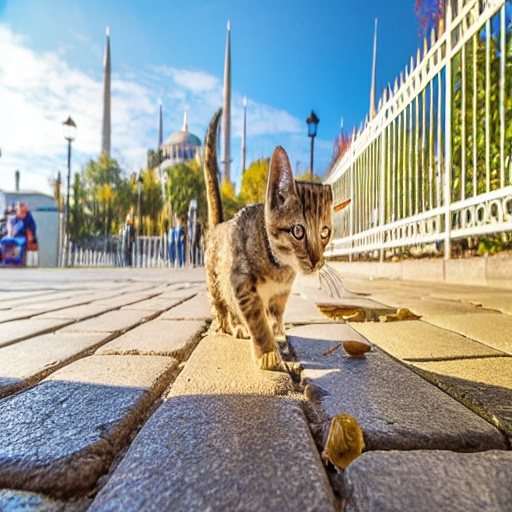
\includegraphics[width=0.32\linewidth]{cat_source.jpg} &
        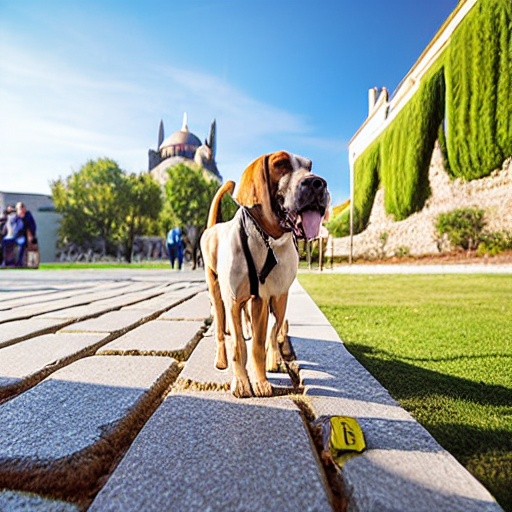
\includegraphics[width=0.32\linewidth]{cat_all_ones.jpg} &
        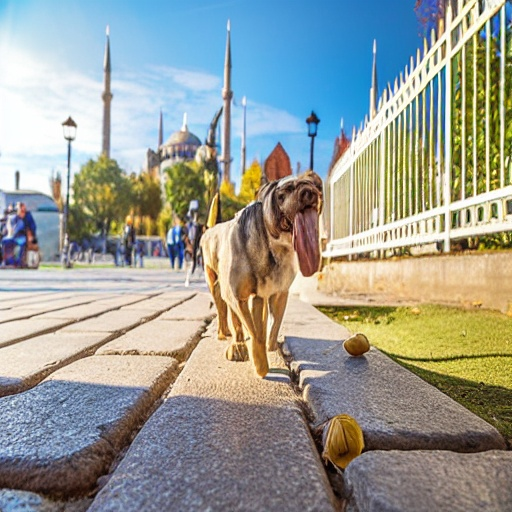
\includegraphics[width=0.32\linewidth]{cat_best.jpg} \\[-0.1em]
        {\tiny source} & {\tiny all-target} & {\tiny good edit}\\[0.3em]
        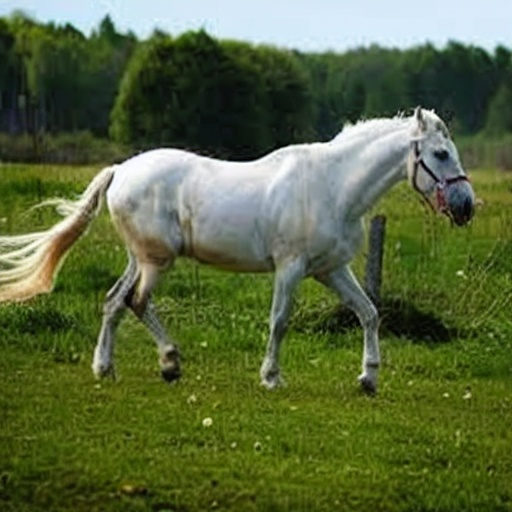
\includegraphics[width=0.32\linewidth]{horse_source.jpg} &
        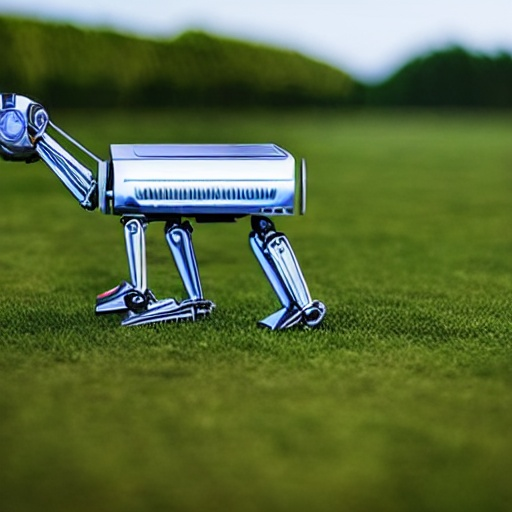
\includegraphics[width=0.32\linewidth]{horse_all_ones.jpg} &
        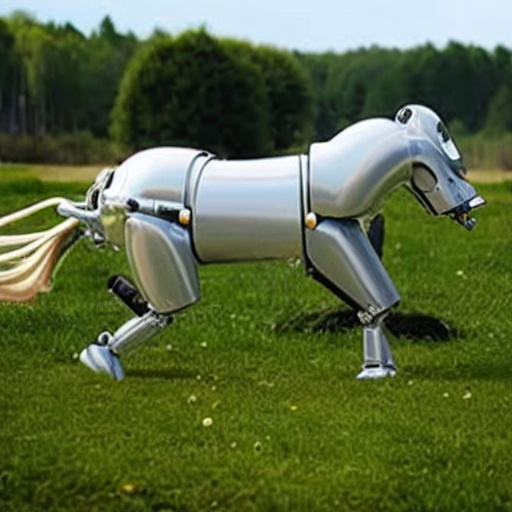
\includegraphics[width=0.32\linewidth]{horse_best.jpg} \\[-0.1em]
        {\tiny source} & {\tiny all-target} & {\tiny good edit}\\
      \end{tabular}
    \end{column}
  \end{columns}
\end{frame}

% 3 ==== Reward ============================================================
\begin{frame}{A reward for the two objectives}
  \vspace{0.4em}
  \Large
  \begin{itemize}
    \item \key{Background score} \; $f_\text{bg}$ \\[0.2em]
          similarity of the new image to the source on background pixels only.
    \vspace{0.6em}
    \item \key{Prompt score} \; $f_\text{fg}$ \\[0.2em]
          does the foreground match ``target minus source'' in vision-language space?
  \end{itemize}
  \normalsize

  \vspace{1.2em}
  \begin{center}
    \Large
    $R \;=\; \sqrt{\, f_\text{bg}\,\cdot\, f_\text{fg}\,}$
    \normalsize
  \end{center}

  \vspace{0.5em}
  \centering\small \emph{Geometric mean \textendash\ zero if either side collapses, so both must be met.}
\end{frame}

% 4 ==== Idea: exploit diffusion diversity =================================
\begin{frame}{Idea \textendash\ exploit the network's own diversity}
  A diffusion model runs $T$ denoising steps. At each step the latent update depends on the \key{text condition} $c_t$:
  \begin{equation*}
    \mathbf z_{t-1} \;=\; \text{step}\bigl(\mathbf z_t,\, t,\, \textcolor{accent}{c_t}\bigr)
    \qquad\footnotesize\text{(noise prediction or velocity, conditioned on $c_t$)}
  \end{equation*}

  Normally $c_t$ is fixed \textendash\ the same prompt every step. Instead, pick it per step via a binary mask:
  \begin{equation*}
    c_t \;=\; m_t\,\psi(P_\text{tgt}) + (1{-}m_t)\,\psi(P_\text{src}), \qquad M=[m_T,\dots,m_1]\in\{0,1\}^T.
  \end{equation*}

  \begin{itemize}
    \item Each mask $M$ is a \key{trajectory} through the model.
    \item $2^T$ candidate trajectories \textendash\ no weight updates, no inversion.
    \item $M=\mathbf 1$ (all target) is just one point in a huge space.
  \end{itemize}

  \vspace{0.2em}
  \alert{Question:}\; is this space rich and does it contain high-reward trajectories?
\end{frame}

% 5 ==== Motivational exhaustive --- clusters ==============================
\begin{frame}{Motivational experiment \textendash\ the space has structure}
  SD v1.5, enumerate all $2^{20}\!\approx\!10^6$ masks for two probes.
  Cluster outputs by DINOv2+UMAP+HDBSCAN.

  \vspace{0.4em}
  \begin{columns}[T,onlytextwidth]
    \begin{column}{0.48\textwidth}
      \centering
      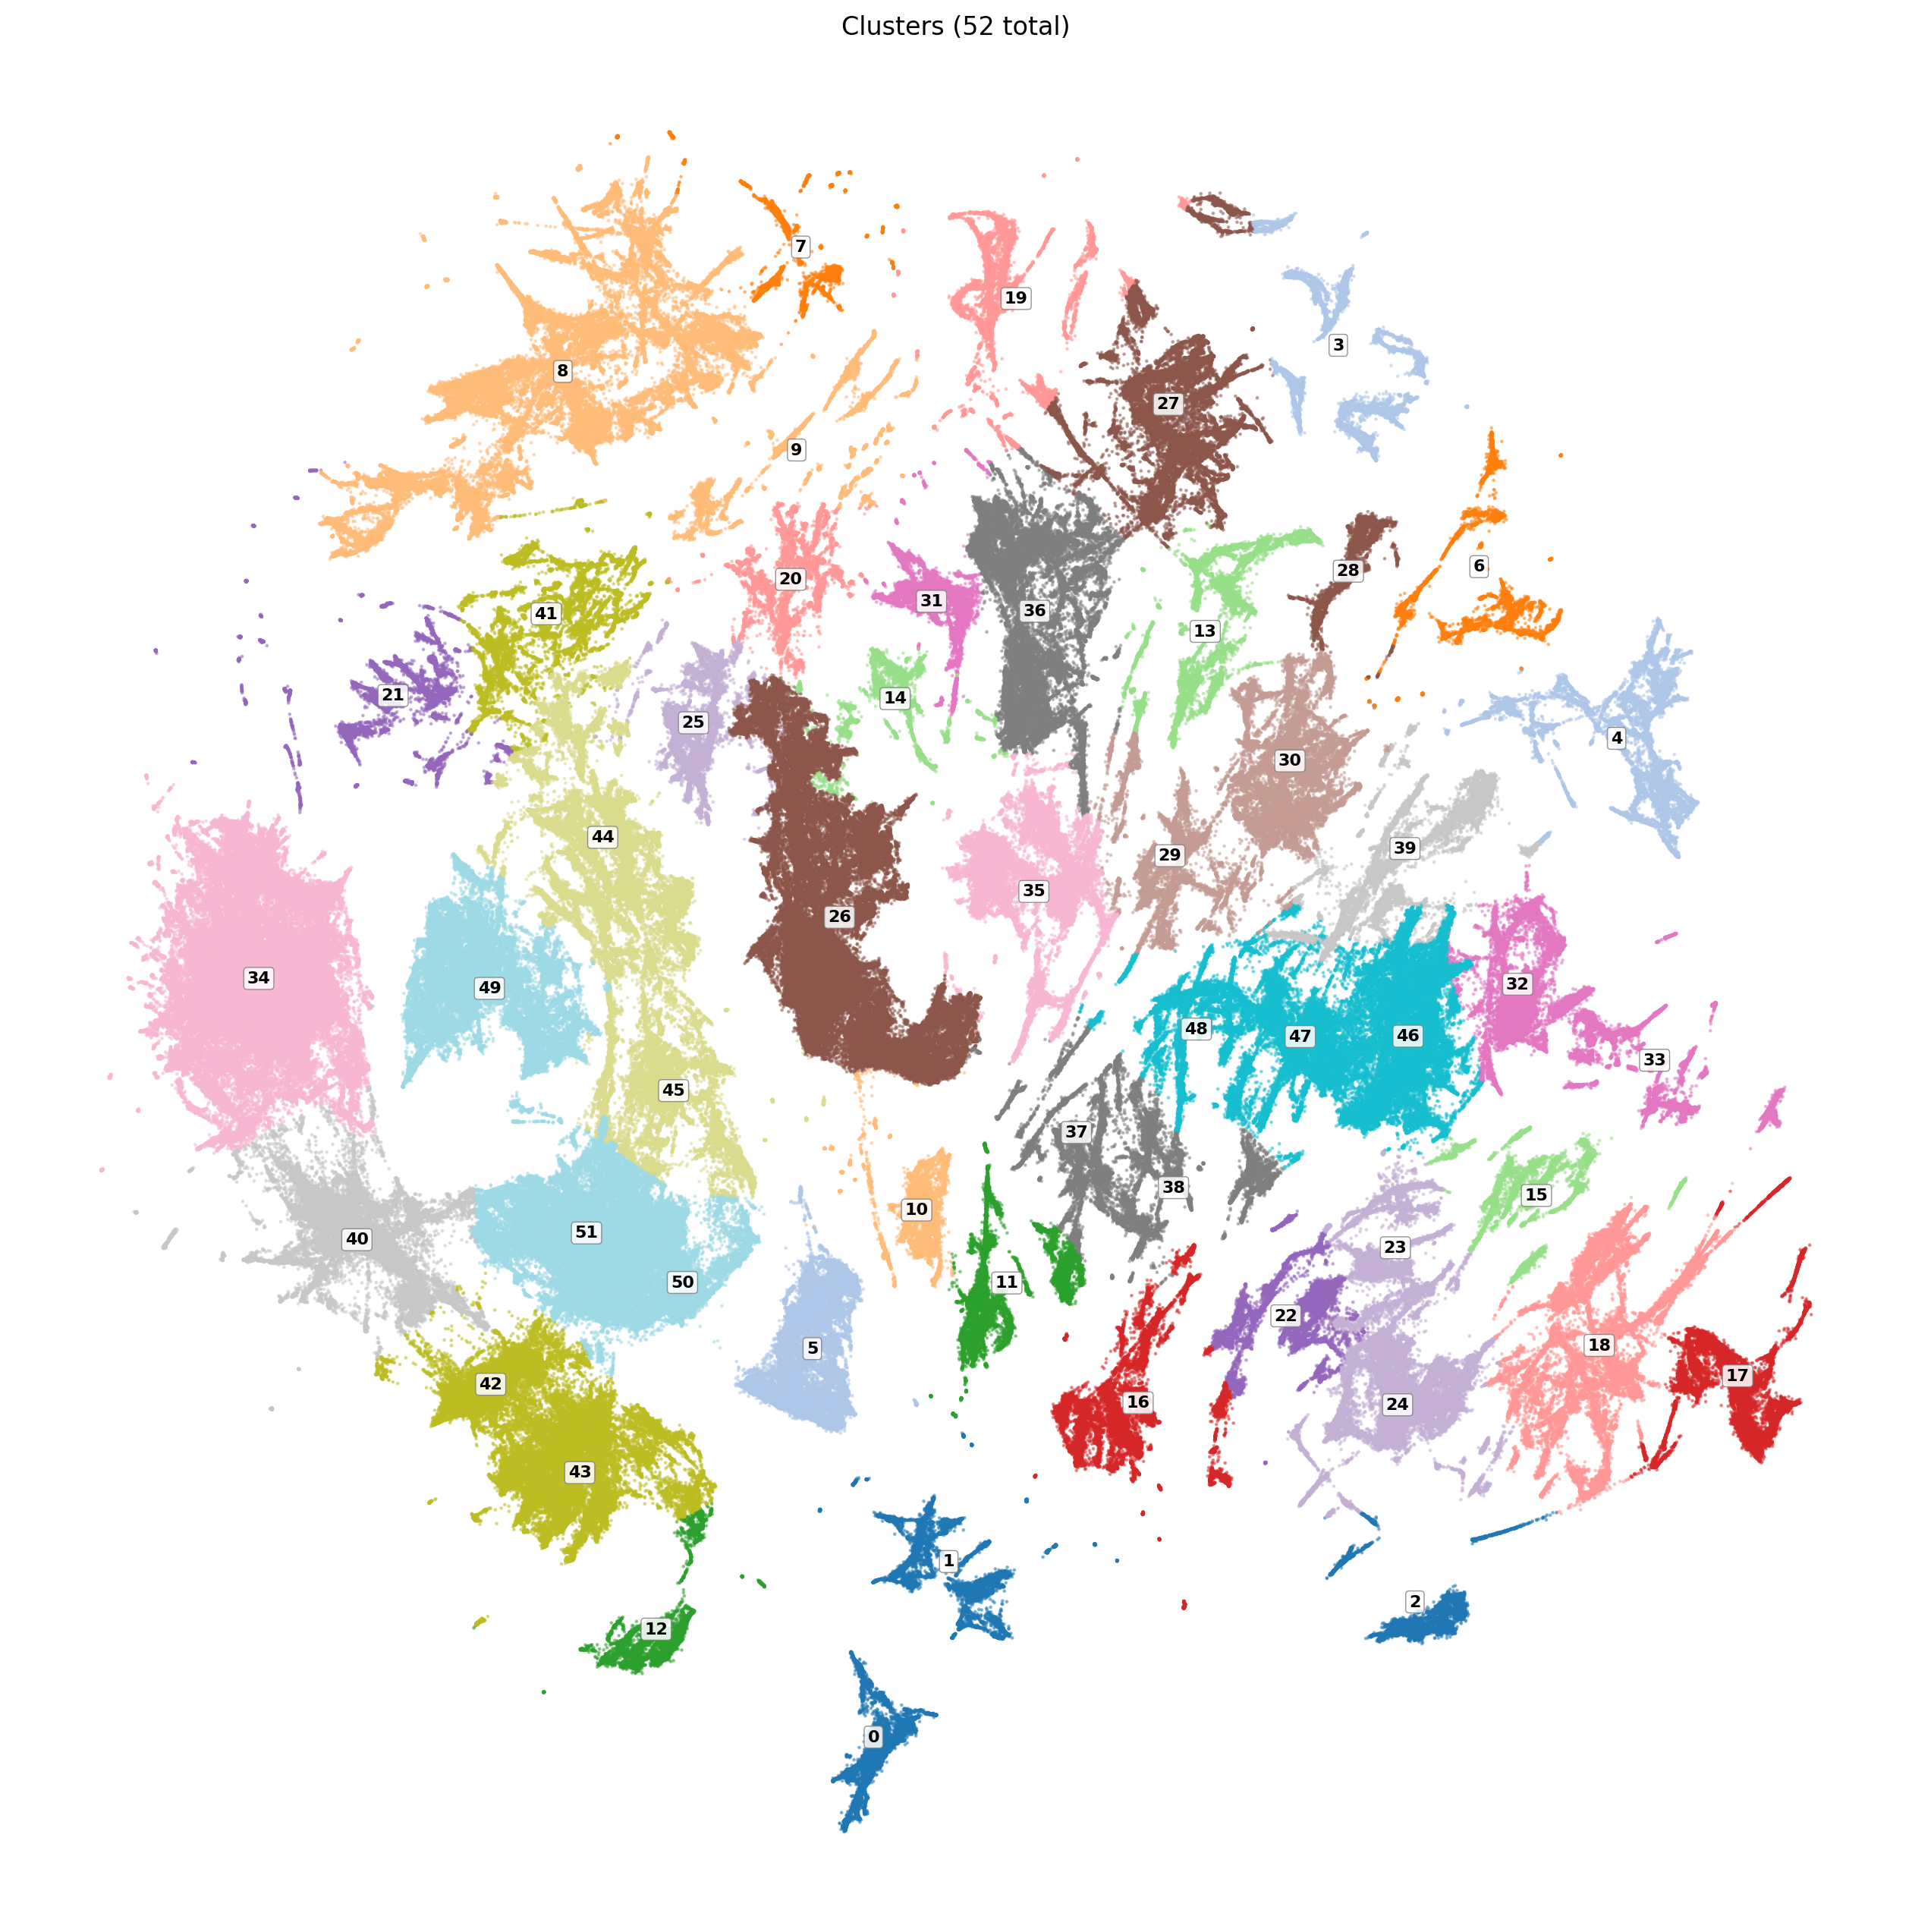
\includegraphics[height=0.56\textheight,keepaspectratio]{catdog_map_clusters.png}\\[-0.2em]
      {\scriptsize cat$\to$dog: \textbf{52} clusters}
    \end{column}
    \begin{column}{0.48\textwidth}
      \centering
      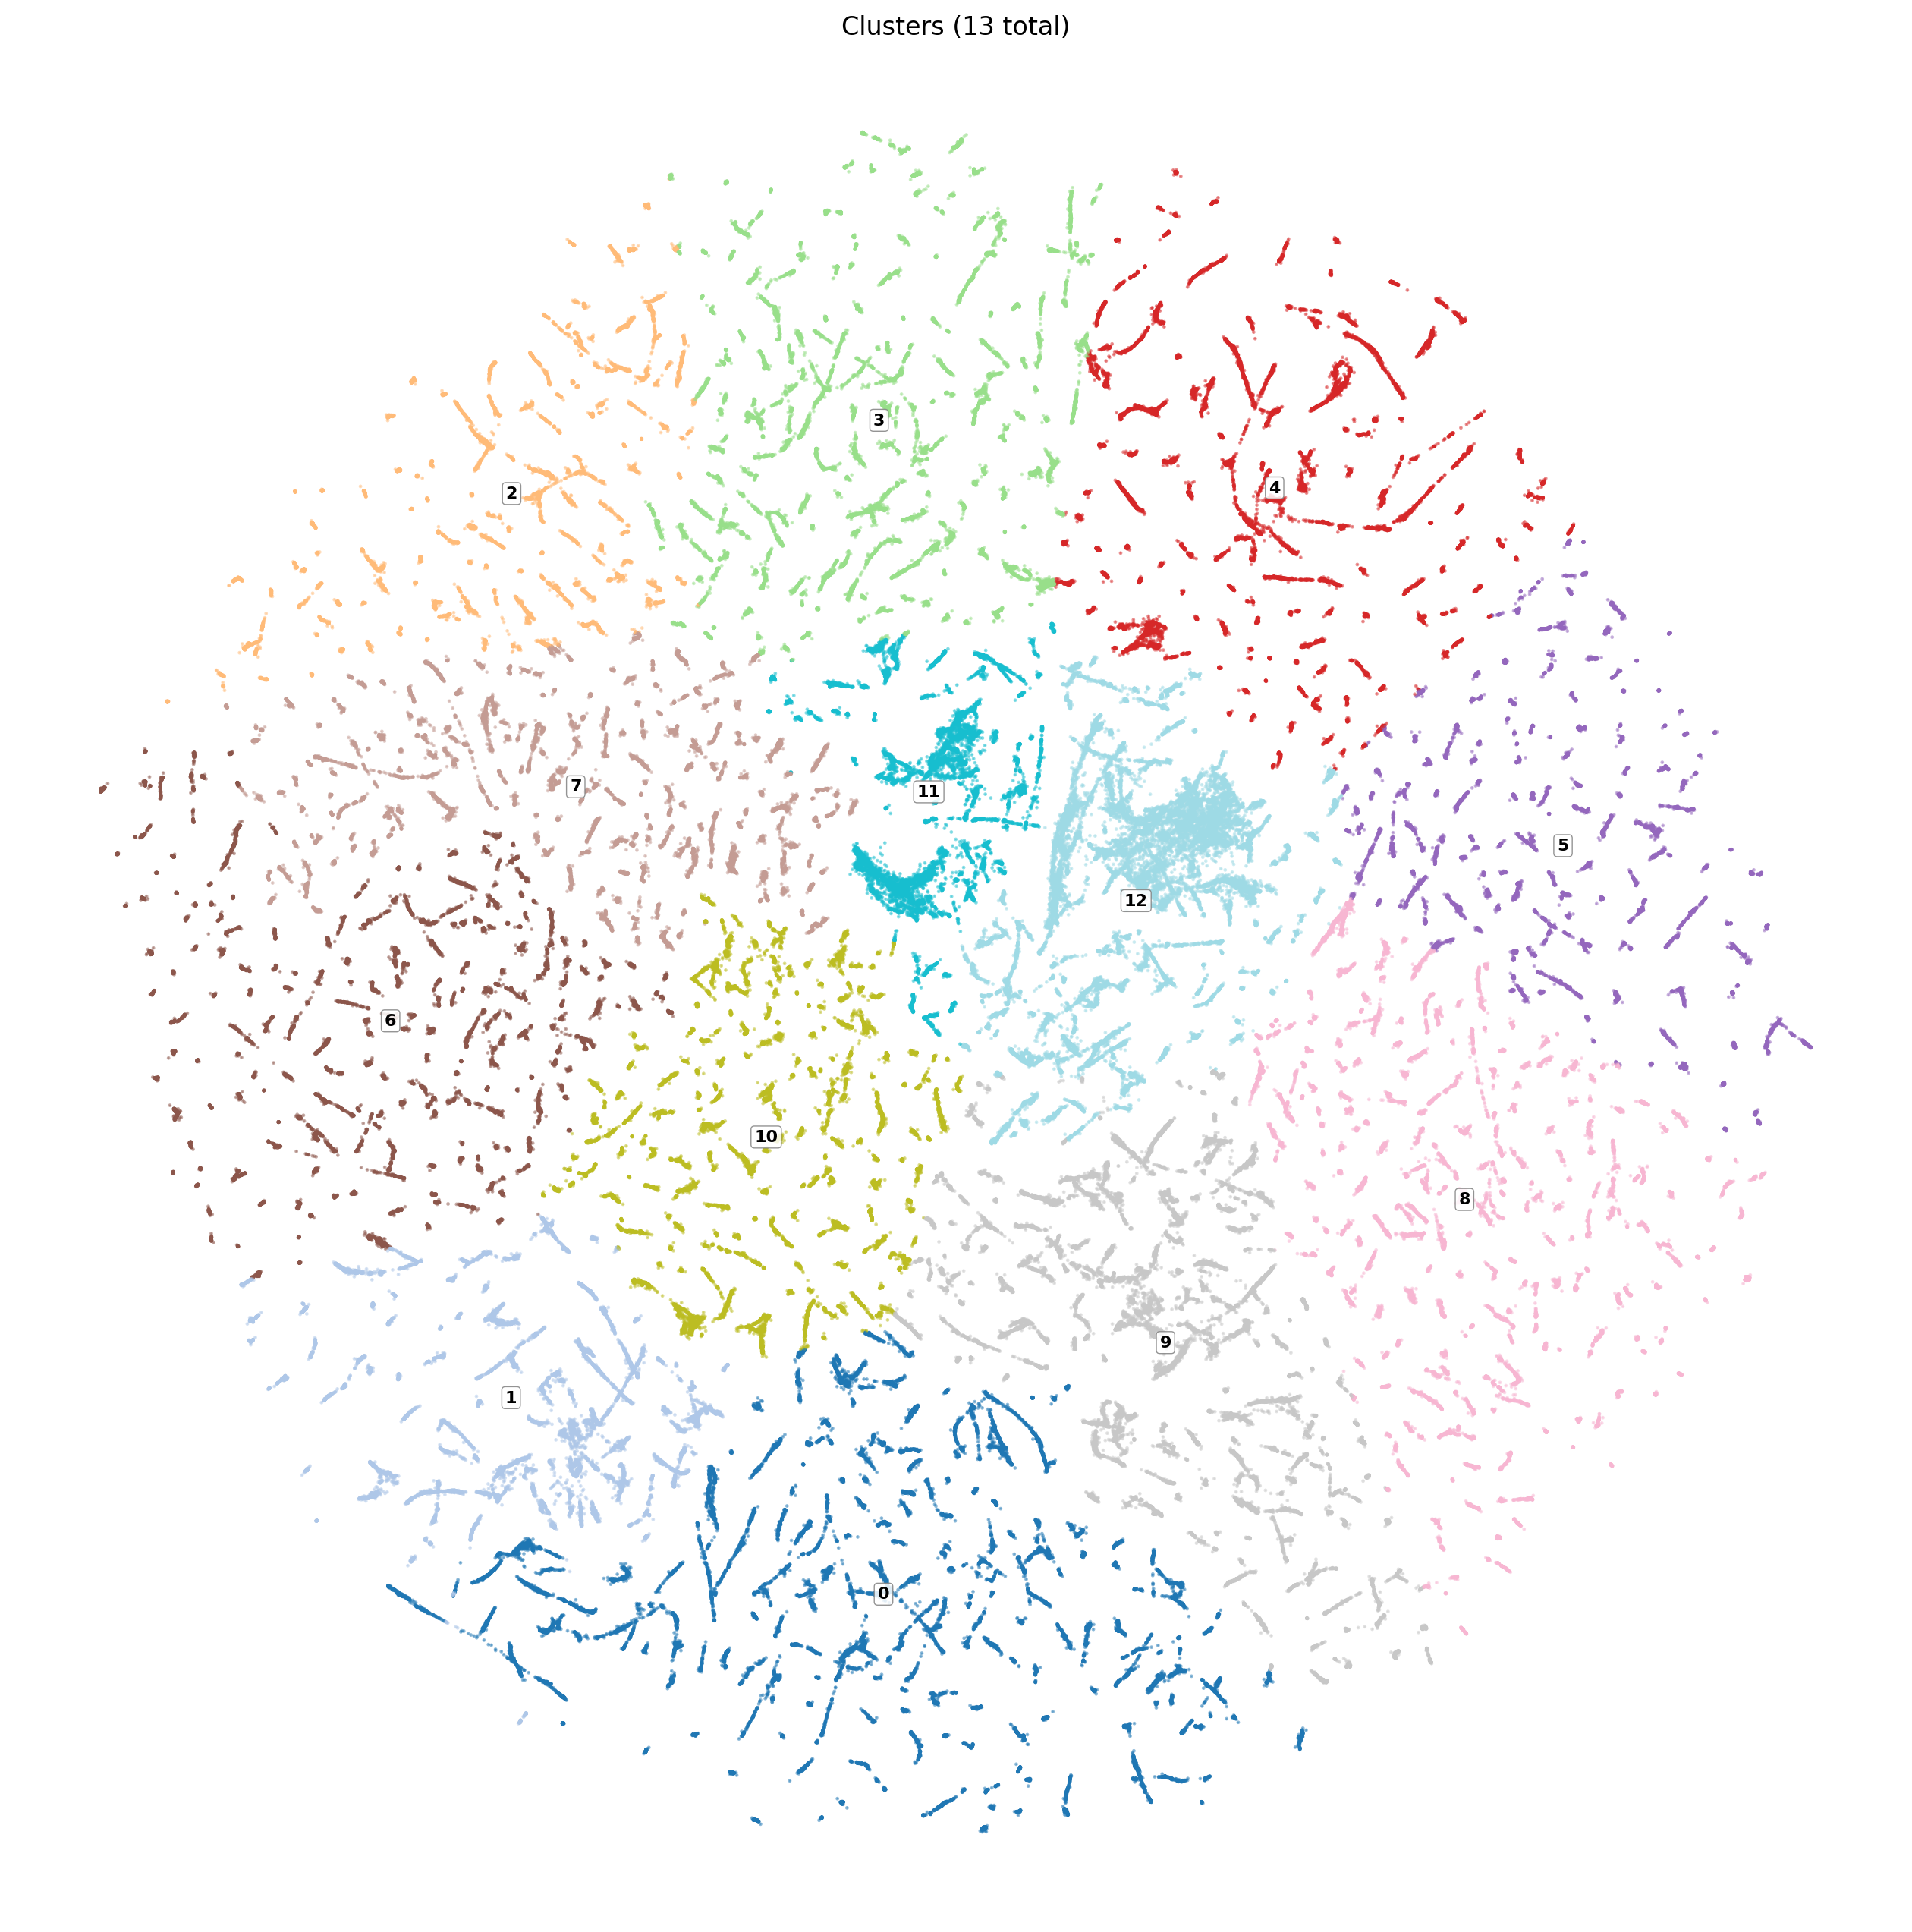
\includegraphics[height=0.56\textheight,keepaspectratio]{horse_map_clusters.png}\\[-0.2em]
      {\scriptsize horse$\to$robot: \textbf{13} clusters}
    \end{column}
  \end{columns}

  \vspace{0.4em}
  \centering\small The mask space breaks into visually distinct groups. \key{Structure exists.}
\end{frame}

% 6 ==== Reward map on UMAP ================================================
\begin{frame}{Reward map \textendash\ high-reward regions are real}
  Same UMAPs, coloured by \emph{combined reward}.

  \vspace{0.3em}
  \begin{columns}[T,onlytextwidth]
    \begin{column}{0.48\textwidth}
      \centering
      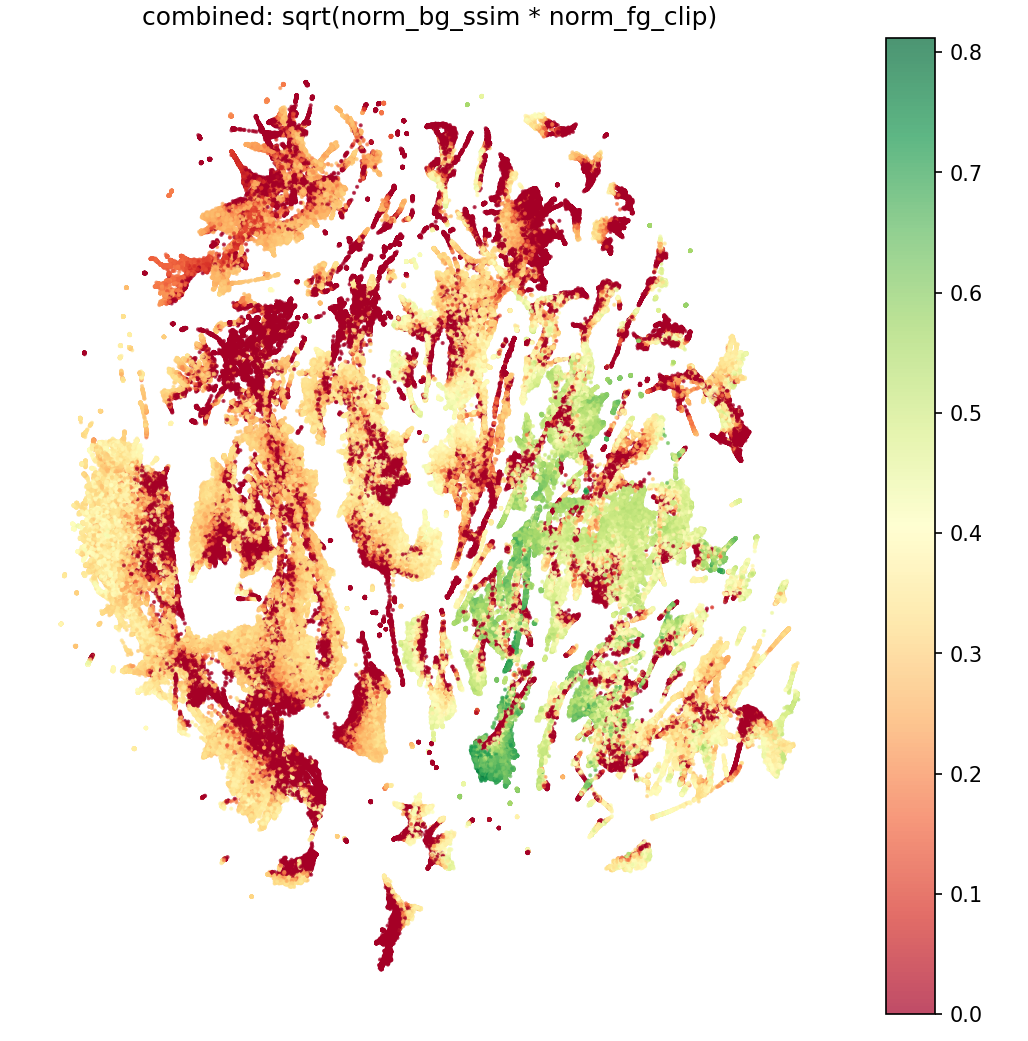
\includegraphics[height=0.58\textheight,keepaspectratio]{catdog_combined_umap.png}\\[-0.2em]
      {\scriptsize cat $\to$ dog}
    \end{column}
    \begin{column}{0.48\textwidth}
      \centering
      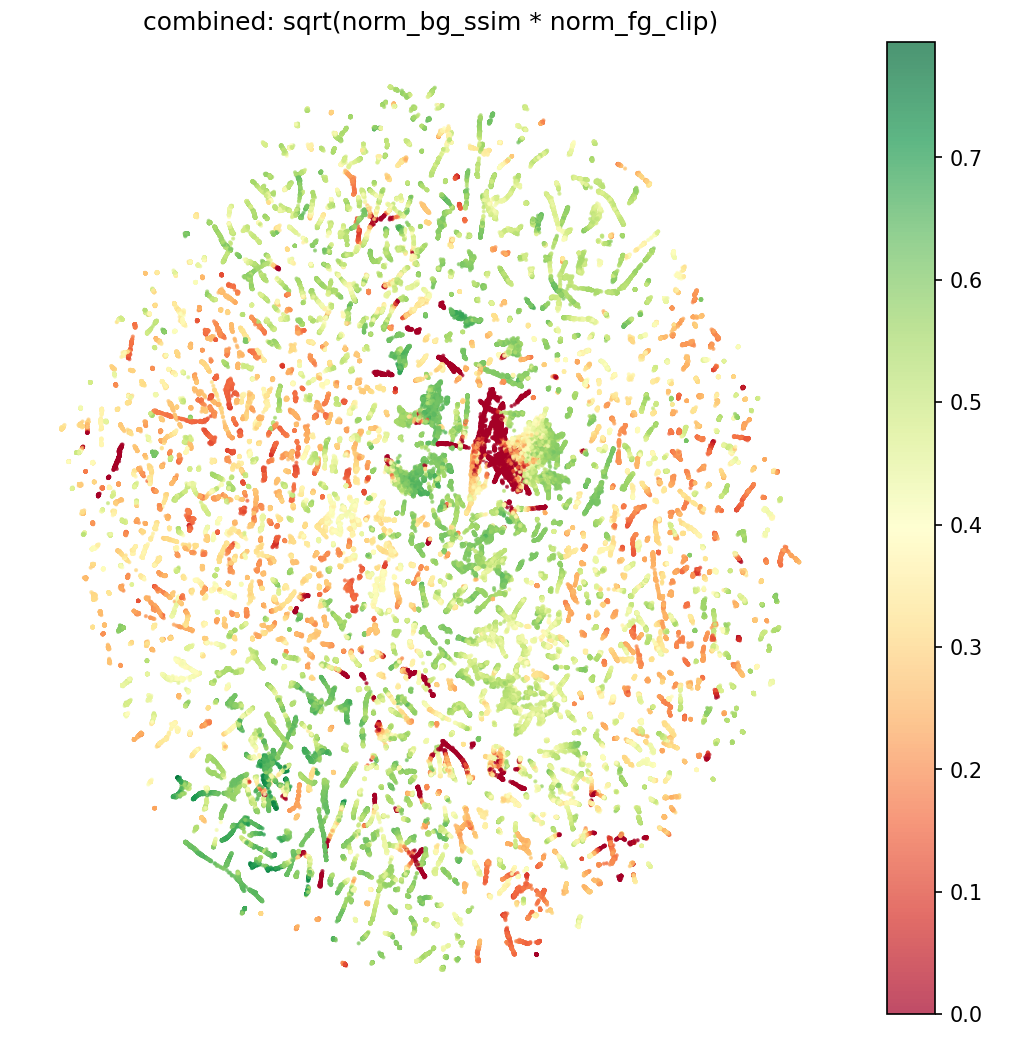
\includegraphics[height=0.58\textheight,keepaspectratio]{horse_combined_umap.png}\\[-0.2em]
      {\scriptsize horse $\to$ robot}
    \end{column}
  \end{columns}

  \vspace{0.3em}
  \centering\small
  \key{High-reward masks cluster in a few regions}, not spread evenly across the space. A search algorithm that lands in any of them is enough.
\end{frame}

% 7 ==== Visual confirmation ===============================================
\begin{frame}{Visual confirmation \textendash\ cluster diversity}
  Six largest clusters per task, 5 representative images each.

  \vspace{0.2em}
  \begin{columns}[T,onlytextwidth]
    \begin{column}{0.48\textwidth}
      \centering
      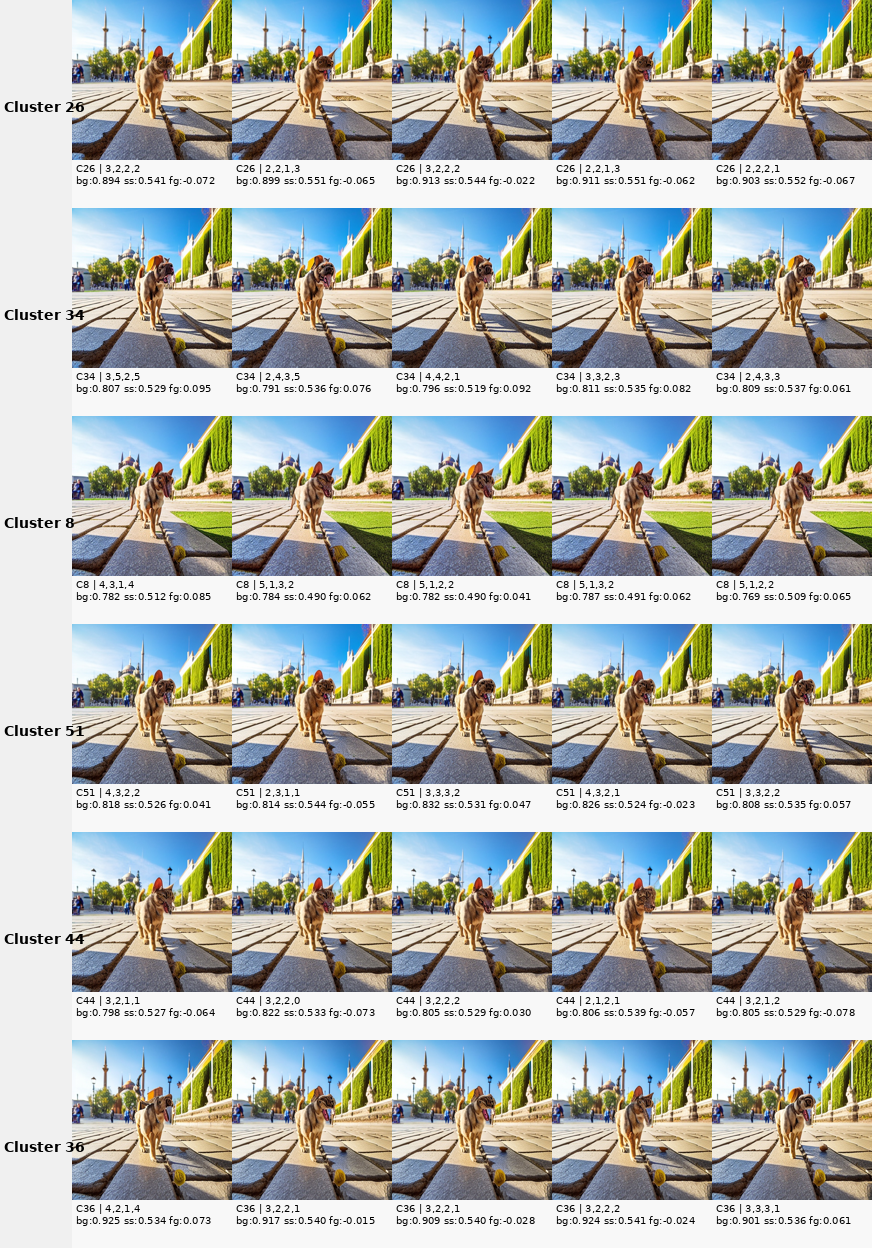
\includegraphics[height=0.68\textheight,keepaspectratio]{catdog_grid_top6_x5.png}\\[-0.2em]
      {\scriptsize cat $\to$ dog}
    \end{column}
    \begin{column}{0.48\textwidth}
      \centering
      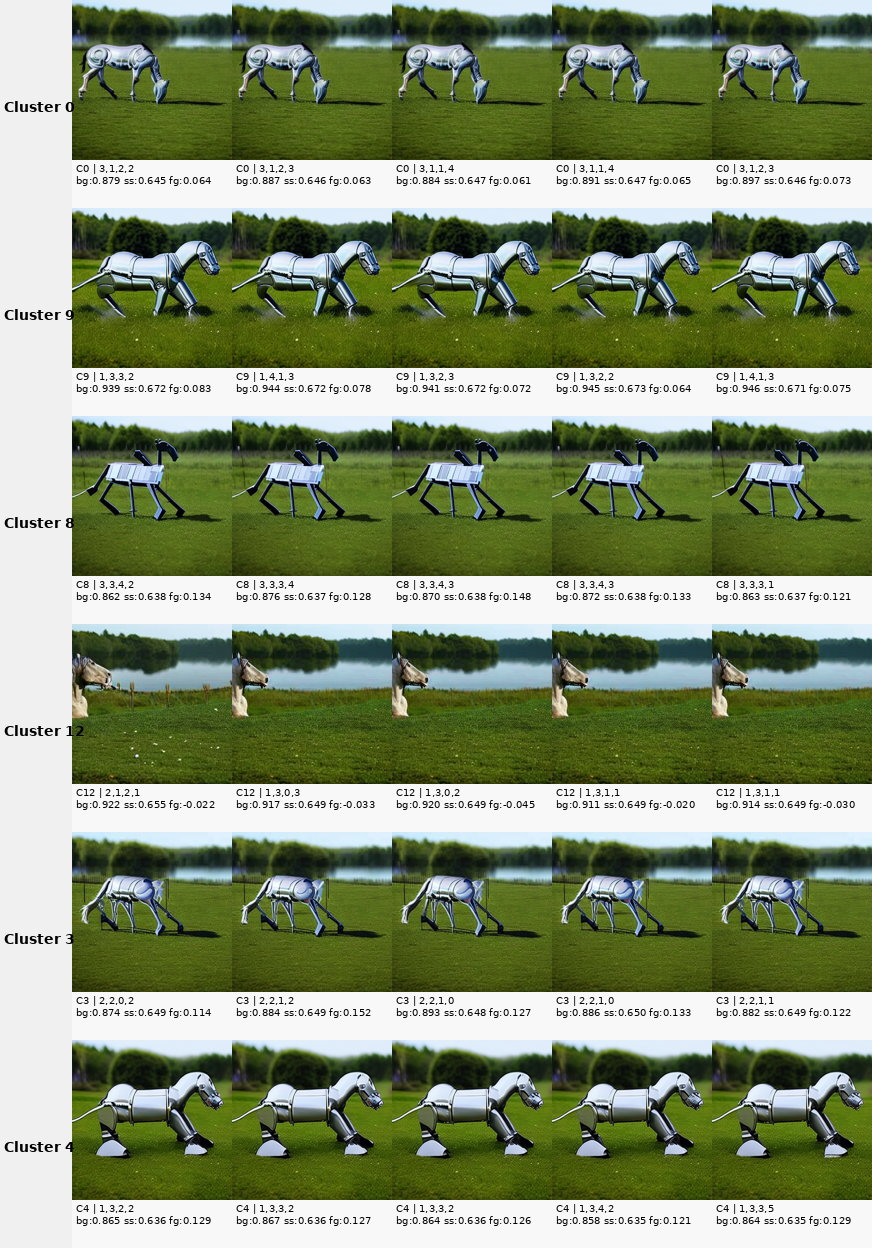
\includegraphics[height=0.68\textheight,keepaspectratio]{horse_grid_top6_x5.png}\\[-0.2em]
      {\scriptsize horse $\to$ robot}
    \end{column}
  \end{columns}
\end{frame}

% 8 ==== Need an algorithm -> REINFORCE ====================================
\begin{frame}{REINFORCE on 14 Bernoulli logits}
  Enumerating $2^{14}=16{,}384$ trajectories is infeasible. We need a search procedure that reaches the high-reward region at a small sampling budget.

  \vspace{0.5em}
  Parameterise the trajectory distribution as independent per-bit Bernoullis and train by REINFORCE:
  \begin{equation*}
    \pi_\theta(M)=\prod_{i=1}^{14}\text{Bern}\bigl(m_i\,\big|\,\sigma(\theta_i)\bigr),\quad
    \mathcal L(\theta) = -\tfrac1K\!\sum_k A^{(k)}\!\sum_i\!\log\pi_\theta\bigl(m_i^{(k)}\bigr) - \beta\, H(\pi_\theta)
  \end{equation*}

  \vspace{0.3em}
  $A^{(k)}$ \textendash\ \key{advantage} of mask $M^{(k)}$: how much its reward beats the running average, normalised across the batch.
  \begin{equation*}
    A^{(k)} \;=\; \frac{R\bigl(M^{(k)}\bigr) - b}{\mathrm{std}_k\,R + 10^{-6}},\qquad
    b \leftarrow 0.9\,b + 0.1\,\overline{R},\quad
    \overline{R}=\tfrac{1}{K}\!\sum_{k}\!R\bigl(M^{(k)}\bigr)
  \end{equation*}

  \vspace{0.1em}
  \small Masks with $A^{(k)}>0$ are reinforced, with $A^{(k)}<0$ suppressed. The entropy term $\beta H(\pi_\theta)$ keeps the policy from collapsing too early.
\end{frame}

% 9 ==== 8 experiments --- REINFORCE vs baseline vs random =================
\begin{frame}{REINFORCE beats baseline and random (8 edits)}
  \begin{columns}[T,onlytextwidth]
    \begin{column}{0.68\textwidth}
      \centering
      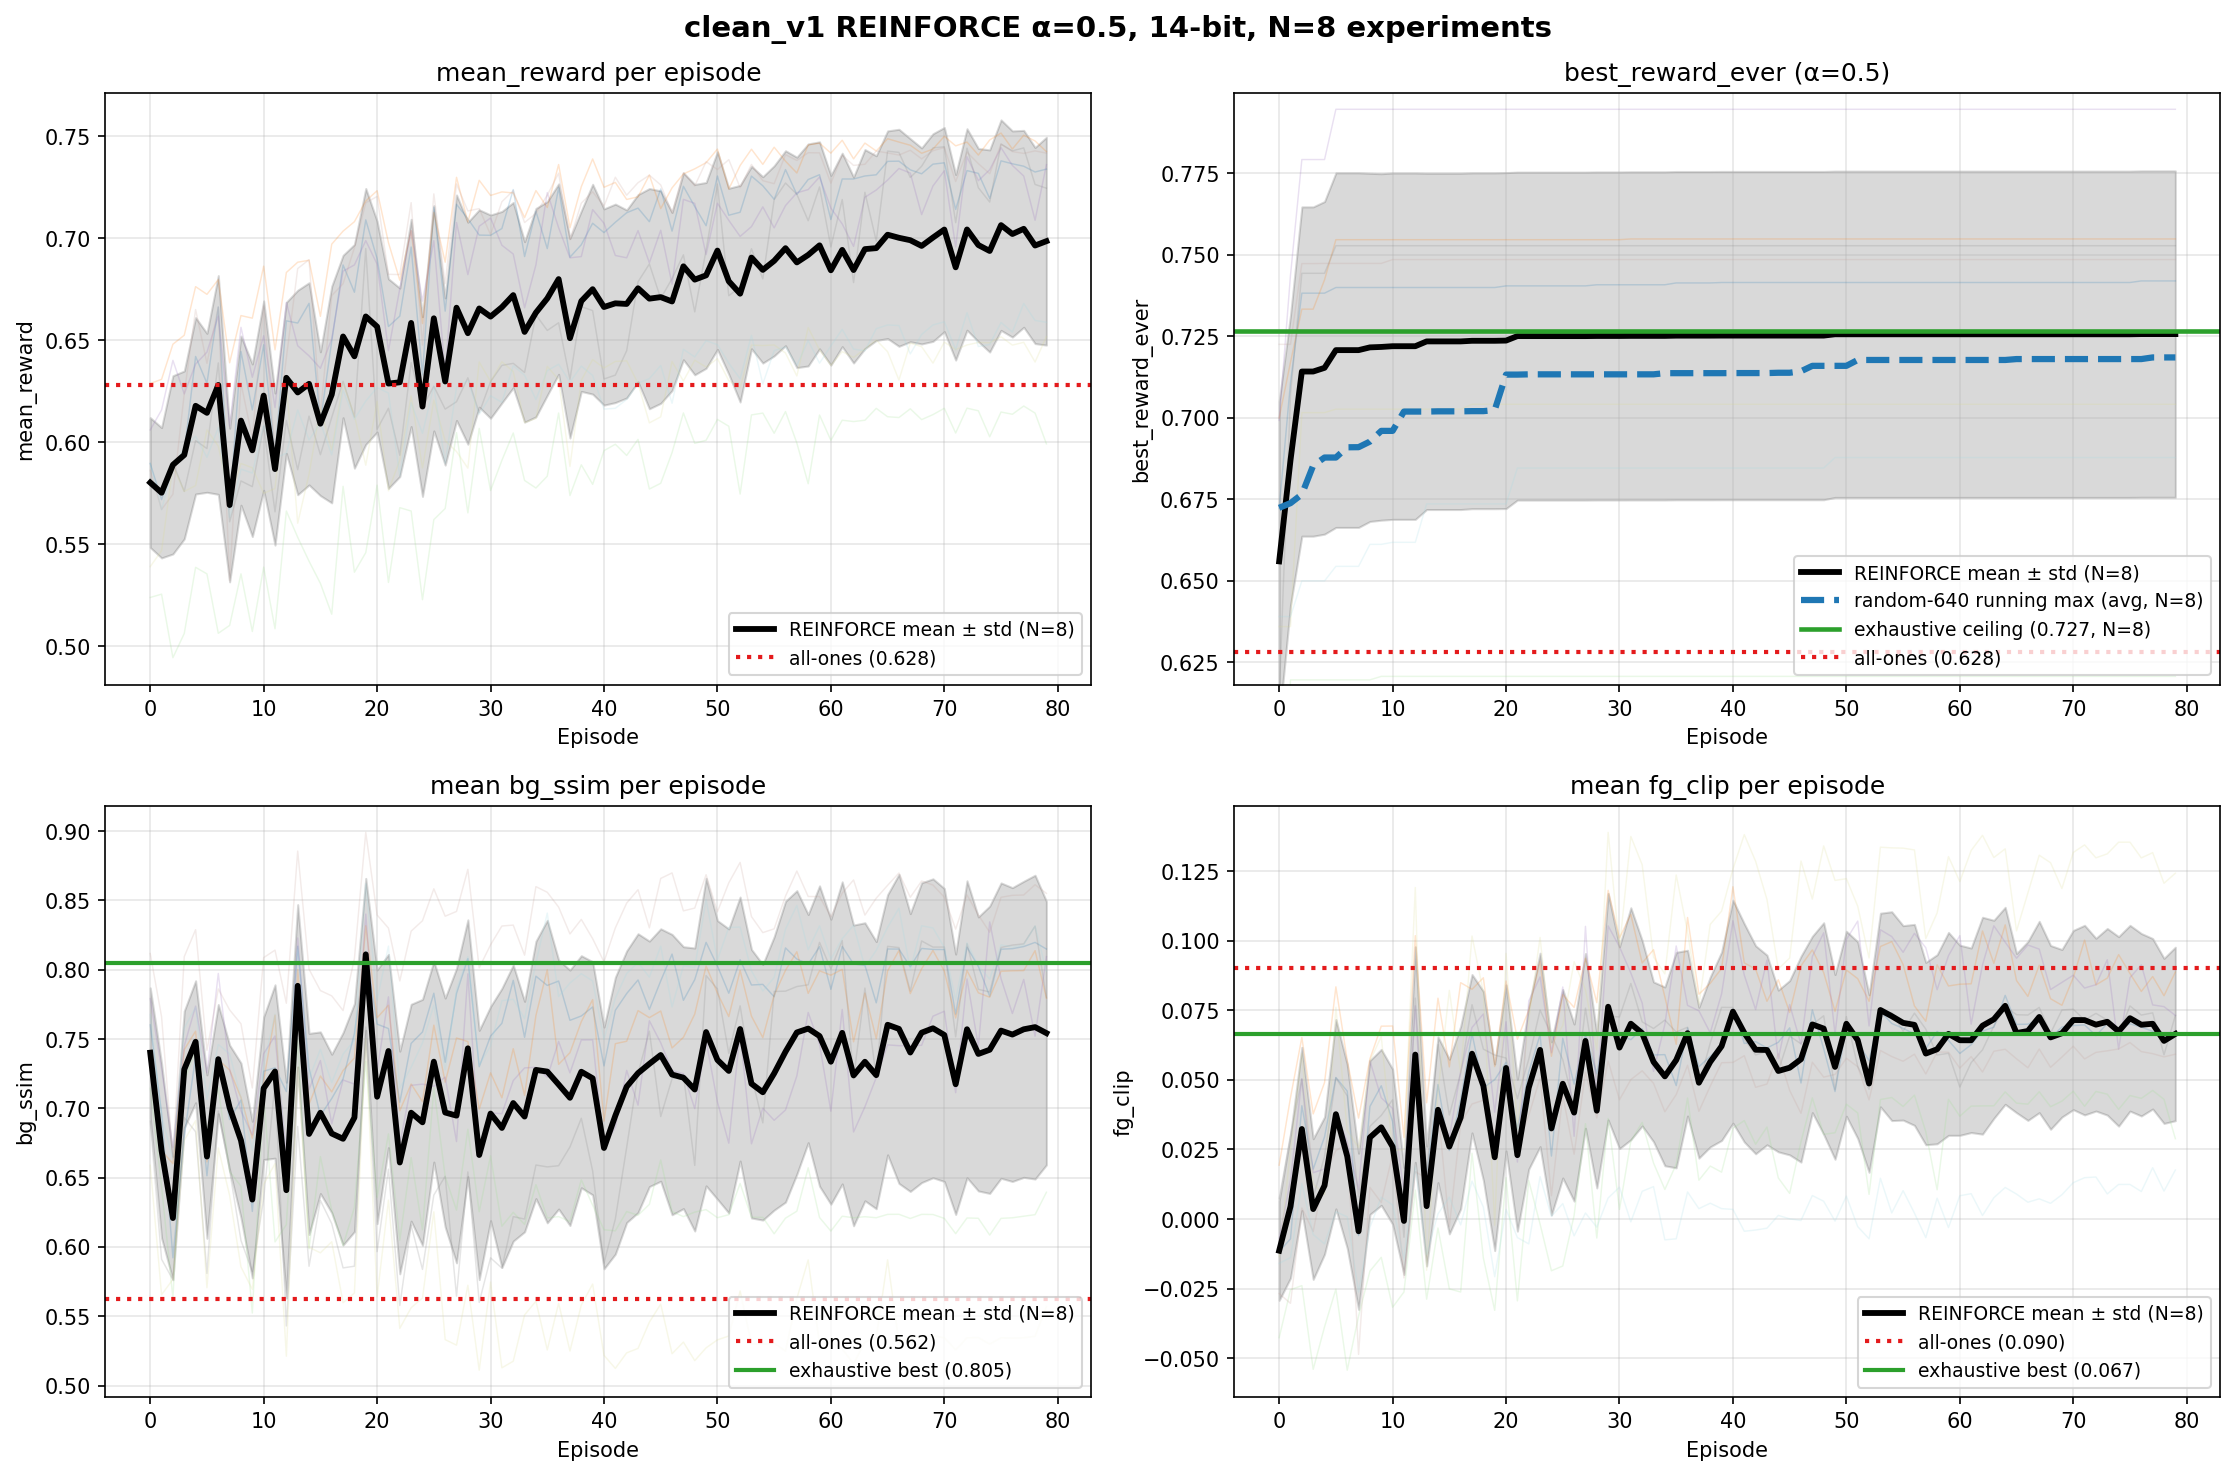
\includegraphics[width=\linewidth,height=0.78\textheight,keepaspectratio]{clean_v1_training_curves.png}
    \end{column}
    \begin{column}{0.30\textwidth}
      \vspace{0.3em}
      \textbf{Learned policy}\\
      reaches a reward\\
      of \textcolor{accent}{\textbf{0.749}} on average.

      \vspace{0.9em}
      \textbf{Baseline} (all-target\\ mask): 0.601.

      \vspace{0.9em}
      REINFORCE wins on\\
      \key{every edit} against
      \begin{itemize}\small
        \item the all-target baseline,
        \item random search at the same sampling budget.
      \end{itemize}
    \end{column}
  \end{columns}
\end{frame}

% 10 ==== Ceiling ===========================================================
\begin{frame}{How close to the $2^{14}$ ceiling?}
  For each of the 8 edits we also ran the full $2^{14}$ enumeration, giving a true maximum reward.

  \vspace{0.5em}
  \centering\small
  \begin{tabular}{lccc}
    \toprule
    edit & exhaustive max & REINFORCE@640 & ratio \\
    \midrule
    chess $\to$ checkers         & 0.755 & 0.755 & \textbf{100.0\,\%} \\
    teapot $\to$ samovar         & 0.753 & 0.753 & \textbf{100.0\,\%} \\
    pocketwatch $\to$ compass    & 0.749 & 0.749 & \textbf{100.0\,\%} \\
    camera $\to$ binoculars      & 0.742 & 0.742 & \textbf{100.0\,\%} \\
    guitar $\to$ banjo           & 0.796 & 0.795 & 99.9\,\% \\
    violin $\to$ cello           & 0.689 & 0.688 & 99.9\,\% \\
    telescope $\to$ microscope   & 0.707 & 0.704 & 99.7\,\% \\
    globe $\to$ orrery           & 0.623 & 0.621 & 99.6\,\% \\
    \bottomrule
  \end{tabular}

  \vspace{0.6em}\centering
  REINFORCE at 640 gen reaches \key{99.6\textendash100\,\%} of the exhaustive ceiling.
\end{frame}

% 11 ==== Visual comparison =================================================
\begin{frame}{Visualisation \textendash\ random vs.\ REINFORCE vs.\ exhaustive}
  \centering
  \includegraphics[width=0.96\linewidth,height=0.74\textheight,keepaspectratio]{rand_vs_rl_budget80.png}
\end{frame}

% 12 ==== Conclusion ========================================================
\begin{frame}{Conclusions}
  \begin{itemize}
    \item \key{Diffusion trajectories are diverse.} $2^{20}$ masks split into 52 / 13 visually distinct clusters on SD v1.5.
    \item \key{High-reward regions exist} and are visible on the UMAP reward map.
    \item \key{REINFORCE finds them at low cost.} 640 generations per edit reach 99.6\textendash100\,\% of the $2^{14}$ exhaustive ceiling on all 8 canonical tasks.
    \item Beats both the all-target baseline and matched-budget random on 8 / 8 edits.
  \end{itemize}

  \vspace{1.2em}
  \begin{center}
    {\Large\bfseries Thank you.}\\[0.4em]
    \textcolor{accent}{\rule{0.18\textwidth}{1.2pt}}\\[0.5em]
    {\normalsize Questions?}
  \end{center}
\end{frame}

\end{document}
